% Options for packages loaded elsewhere
\PassOptionsToPackage{unicode}{hyperref}
\PassOptionsToPackage{hyphens}{url}
\PassOptionsToPackage{dvipsnames,svgnames,x11names}{xcolor}
%
\documentclass[
  letterpaper,
  DIV=11,
  numbers=noendperiod,
  paper=6in:9in,
  pagesize=pdftex,
  headinclude=on,
  footinclude=on,
  12pt]{scrreprt}

\usepackage{amsmath,amssymb}
\usepackage{iftex}
\ifPDFTeX
  \usepackage[T1]{fontenc}
  \usepackage[utf8]{inputenc}
  \usepackage{textcomp} % provide euro and other symbols
\else % if luatex or xetex
  \usepackage{unicode-math}
  \defaultfontfeatures{Scale=MatchLowercase}
  \defaultfontfeatures[\rmfamily]{Ligatures=TeX,Scale=1}
\fi
\usepackage{lmodern}
\ifPDFTeX\else  
    % xetex/luatex font selection
\fi
% Use upquote if available, for straight quotes in verbatim environments
\IfFileExists{upquote.sty}{\usepackage{upquote}}{}
\IfFileExists{microtype.sty}{% use microtype if available
  \usepackage[]{microtype}
  \UseMicrotypeSet[protrusion]{basicmath} % disable protrusion for tt fonts
}{}
\makeatletter
\@ifundefined{KOMAClassName}{% if non-KOMA class
  \IfFileExists{parskip.sty}{%
    \usepackage{parskip}
  }{% else
    \setlength{\parindent}{0pt}
    \setlength{\parskip}{6pt plus 2pt minus 1pt}}
}{% if KOMA class
  \KOMAoptions{parskip=half}}
\makeatother
\usepackage{xcolor}
\setlength{\emergencystretch}{3em} % prevent overfull lines
\setcounter{secnumdepth}{5}
% Make \paragraph and \subparagraph free-standing
\ifx\paragraph\undefined\else
  \let\oldparagraph\paragraph
  \renewcommand{\paragraph}[1]{\oldparagraph{#1}\mbox{}}
\fi
\ifx\subparagraph\undefined\else
  \let\oldsubparagraph\subparagraph
  \renewcommand{\subparagraph}[1]{\oldsubparagraph{#1}\mbox{}}
\fi


\providecommand{\tightlist}{%
  \setlength{\itemsep}{0pt}\setlength{\parskip}{0pt}}\usepackage{longtable,booktabs,array}
\usepackage{calc} % for calculating minipage widths
% Correct order of tables after \paragraph or \subparagraph
\usepackage{etoolbox}
\makeatletter
\patchcmd\longtable{\par}{\if@noskipsec\mbox{}\fi\par}{}{}
\makeatother
% Allow footnotes in longtable head/foot
\IfFileExists{footnotehyper.sty}{\usepackage{footnotehyper}}{\usepackage{footnote}}
\makesavenoteenv{longtable}
\usepackage{graphicx}
\makeatletter
\def\maxwidth{\ifdim\Gin@nat@width>\linewidth\linewidth\else\Gin@nat@width\fi}
\def\maxheight{\ifdim\Gin@nat@height>\textheight\textheight\else\Gin@nat@height\fi}
\makeatother
% Scale images if necessary, so that they will not overflow the page
% margins by default, and it is still possible to overwrite the defaults
% using explicit options in \includegraphics[width, height, ...]{}
\setkeys{Gin}{width=\maxwidth,height=\maxheight,keepaspectratio}
% Set default figure placement to htbp
\makeatletter
\def\fps@figure{htbp}
\makeatother
\newlength{\cslhangindent}
\setlength{\cslhangindent}{1.5em}
\newlength{\csllabelwidth}
\setlength{\csllabelwidth}{3em}
\newlength{\cslentryspacingunit} % times entry-spacing
\setlength{\cslentryspacingunit}{\parskip}
\newenvironment{CSLReferences}[2] % #1 hanging-ident, #2 entry spacing
 {% don't indent paragraphs
  \setlength{\parindent}{0pt}
  % turn on hanging indent if param 1 is 1
  \ifodd #1
  \let\oldpar\par
  \def\par{\hangindent=\cslhangindent\oldpar}
  \fi
  % set entry spacing
  \setlength{\parskip}{#2\cslentryspacingunit}
 }%
 {}
\usepackage{calc}
\newcommand{\CSLBlock}[1]{#1\hfill\break}
\newcommand{\CSLLeftMargin}[1]{\parbox[t]{\csllabelwidth}{#1}}
\newcommand{\CSLRightInline}[1]{\parbox[t]{\linewidth - \csllabelwidth}{#1}\break}
\newcommand{\CSLIndent}[1]{\hspace{\cslhangindent}#1}

\usepackage{fvextra}
\DefineVerbatimEnvironment{Highlighting}{Verbatim}{breaklines,commandchars=\\\{\}}
\areaset[0.50in]{4.5in}{8in}
\KOMAoption{captions}{tableheading}
\makeatletter
\makeatother
\makeatletter
\@ifpackageloaded{bookmark}{}{\usepackage{bookmark}}
\makeatother
\makeatletter
\@ifpackageloaded{caption}{}{\usepackage{caption}}
\AtBeginDocument{%
\ifdefined\contentsname
  \renewcommand*\contentsname{Table of contents}
\else
  \newcommand\contentsname{Table of contents}
\fi
\ifdefined\listfigurename
  \renewcommand*\listfigurename{List of Figures}
\else
  \newcommand\listfigurename{List of Figures}
\fi
\ifdefined\listtablename
  \renewcommand*\listtablename{List of Tables}
\else
  \newcommand\listtablename{List of Tables}
\fi
\ifdefined\figurename
  \renewcommand*\figurename{Figure}
\else
  \newcommand\figurename{Figure}
\fi
\ifdefined\tablename
  \renewcommand*\tablename{Table}
\else
  \newcommand\tablename{Table}
\fi
}
\@ifpackageloaded{float}{}{\usepackage{float}}
\floatstyle{ruled}
\@ifundefined{c@chapter}{\newfloat{codelisting}{h}{lop}}{\newfloat{codelisting}{h}{lop}[chapter]}
\floatname{codelisting}{Listing}
\newcommand*\listoflistings{\listof{codelisting}{List of Listings}}
\makeatother
\makeatletter
\@ifpackageloaded{caption}{}{\usepackage{caption}}
\@ifpackageloaded{subcaption}{}{\usepackage{subcaption}}
\makeatother
\makeatletter
\@ifpackageloaded{tcolorbox}{}{\usepackage[skins,breakable]{tcolorbox}}
\makeatother
\makeatletter
\@ifundefined{shadecolor}{\definecolor{shadecolor}{rgb}{.97, .97, .97}}
\makeatother
\makeatletter
\makeatother
\makeatletter
\makeatother
\ifLuaTeX
  \usepackage{selnolig}  % disable illegal ligatures
\fi
\IfFileExists{bookmark.sty}{\usepackage{bookmark}}{\usepackage{hyperref}}
\IfFileExists{xurl.sty}{\usepackage{xurl}}{} % add URL line breaks if available
\urlstyle{same} % disable monospaced font for URLs
\hypersetup{
  pdftitle={टोटलाको फूल},
  pdfauthor={Mohit Shrestha},
  colorlinks=true,
  linkcolor={blue},
  filecolor={Maroon},
  citecolor={Blue},
  urlcolor={Blue},
  pdfcreator={LaTeX via pandoc}}

\title{टोटलाको फूल}
\author{Mohit Shrestha}
\date{August 2, 2023}

\begin{document}
\maketitle
\RecustomVerbatimEnvironment{verbatim}{Verbatim}{
   showspaces = false,
   showtabs = false,
   breaksymbolleft={},
   breaklines
   % Note: setting commandchars=\\\{\} here will cause an error 
}  

\ifdefined\Shaded\renewenvironment{Shaded}{\begin{tcolorbox}[boxrule=0pt, interior hidden, breakable, enhanced, sharp corners, borderline west={3pt}{0pt}{shadecolor}, frame hidden]}{\end{tcolorbox}}\fi

\renewcommand*\contentsname{Table of contents}
{
\hypersetup{linkcolor=}
\setcounter{tocdepth}{2}
\tableofcontents
}
\bookmarksetup{startatroot}

\hypertarget{ux91fux91fux932ux915-ux92bux932}{%
\chapter*{टोटलाको फूल}\label{ux91fux91fux932ux915-ux92bux932}}
\addcontentsline{toc}{chapter}{टोटलाको फूल}

\markboth{टोटलाको फूल}{टोटलाको फूल}

\begin{figure}[H]

{\centering 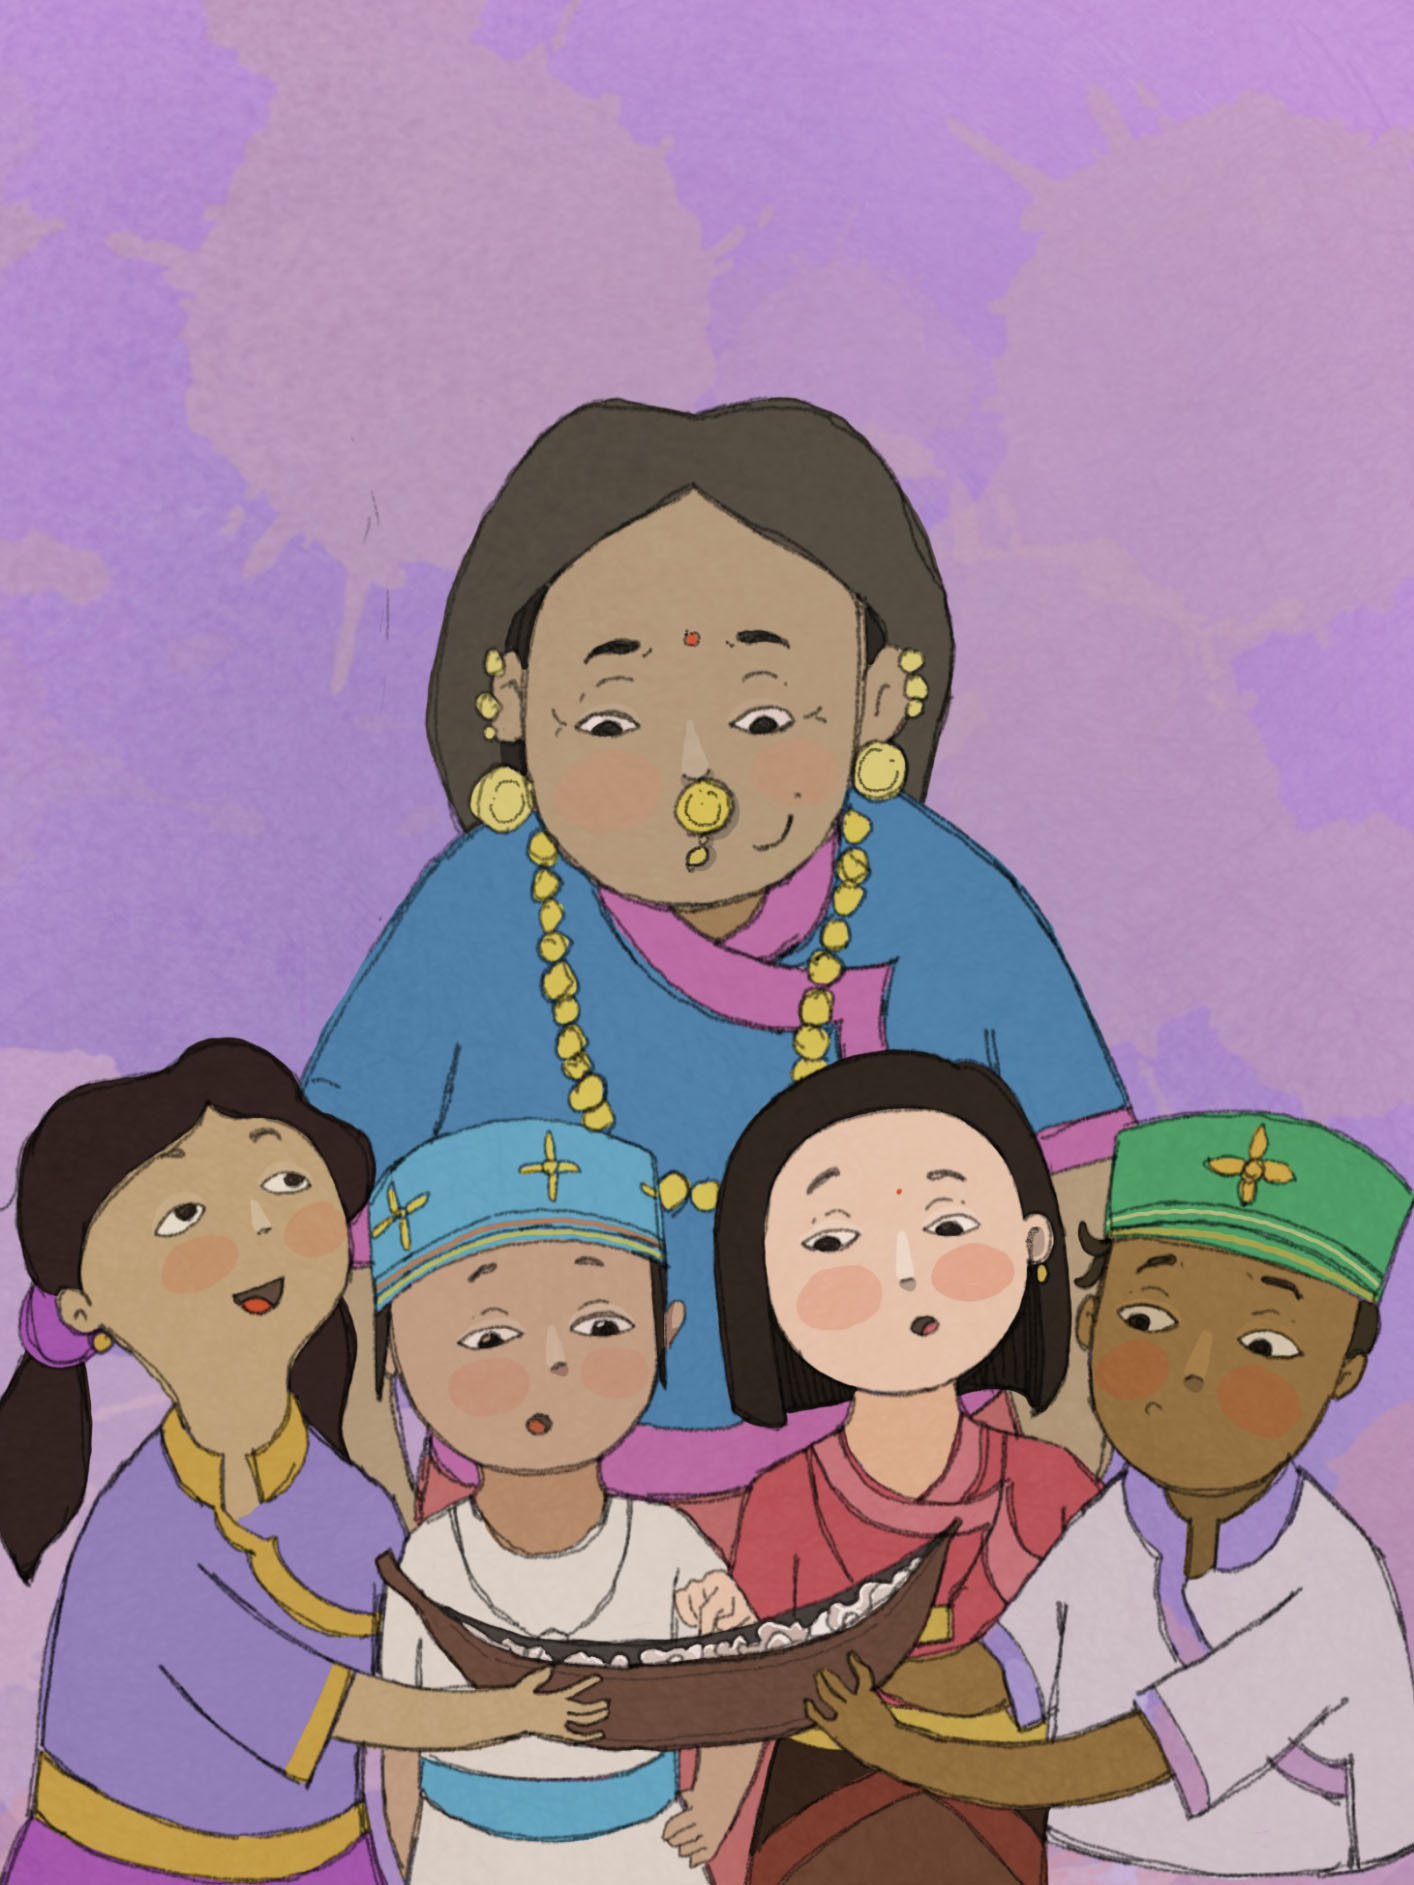
\includegraphics{images/coverImage.jpeg}

}

\end{figure}

\begin{longtable}[]{@{}c@{}}
\toprule\noalign{}
\endhead
\bottomrule\noalign{}
\endlastfoot
\textbf{टोटलाको फूल} \\
\textbf{\emph{Shrijana Gole Tamang}} \\
\textbf{\emph{Suman Maharjan}} \\
\end{longtable}

\begin{figure}[H]

{\centering 
\includegraphics{images/letsread_asf.jpg}

}

\end{figure}

\begin{longtable}[]{@{}
  >{\raggedright\arraybackslash}p{(\columnwidth - 0\tabcolsep) * \real{1.0000}}@{}}
\caption{\textbf{Short Description}}\tabularnewline
\toprule\noalign{}
\endfirsthead
\endhead
\bottomrule\noalign{}
\endlastfoot
साथीहरुसँग खेल्दै गर्दा उर्मुको ध्यान टोटलाको रुखमा पर्छ । त्यो भित्र के होला भनेर !
उर्मुको मनमा कुतकुती हुन्छ र रुखमा चढ्न खोज्दा हजुरआमाले रोक्दै टोटलाको फूलको बारेमा
भन्नुहुन्छ। \\
\end{longtable}

\bookmarksetup{startatroot}

\hypertarget{section}{%
\chapter{}\label{section}}

\begin{figure}[H]

{\centering 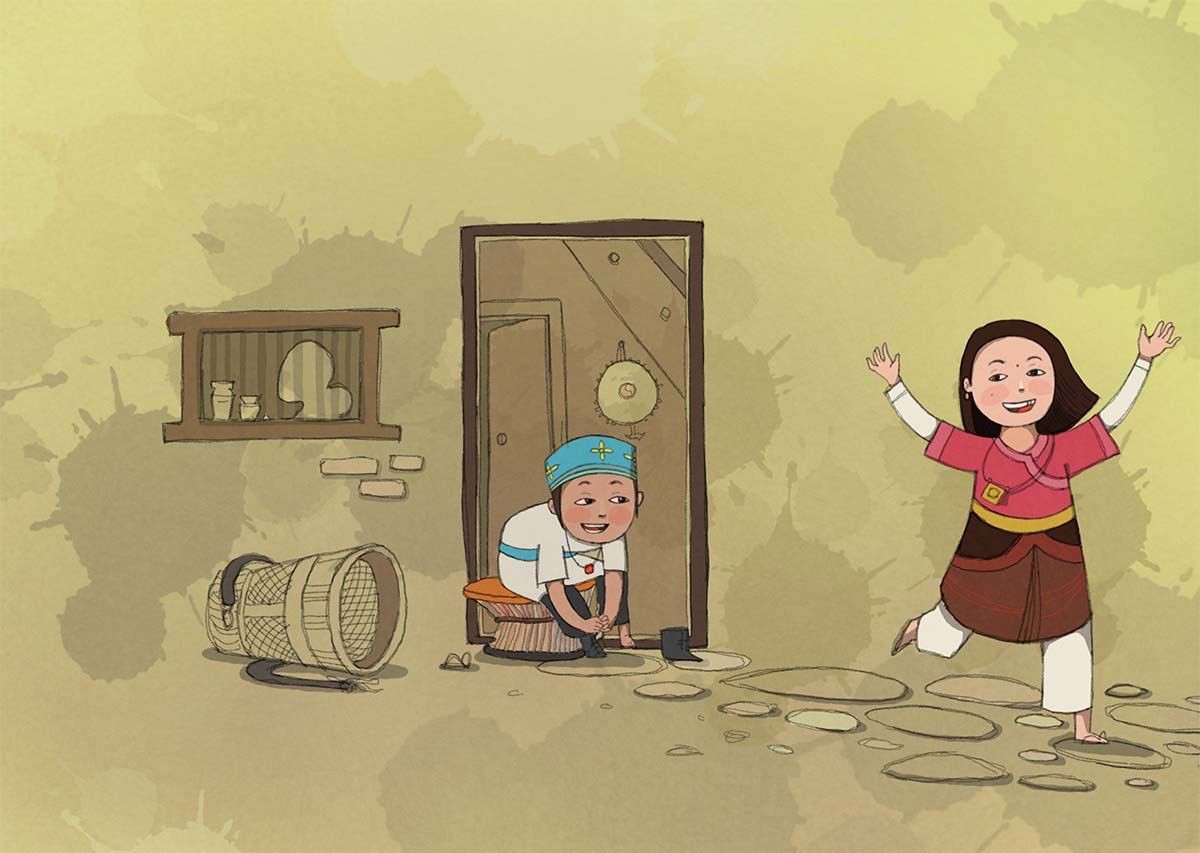
\includegraphics{images/p-2.jpg}

}

\end{figure}

\begin{longtable}[]{@{}
  >{\raggedright\arraybackslash}p{(\columnwidth - 0\tabcolsep) * \real{0.8472}}@{}}
\toprule\noalign{}
\endhead
\bottomrule\noalign{}
\endlastfoot
\begin{minipage}[t]{\linewidth}\raggedright
``ए उर्गेन ! साथीहरू खेल्न आइसके । म जाँदै गर्छु । तिमी छिट्टै आऊ ल !''\\
``ल नाना ल !''\strut
\end{minipage} \\
\end{longtable}

\bookmarksetup{startatroot}

\hypertarget{section-1}{%
\chapter{}\label{section-1}}

\begin{figure}[H]

{\centering 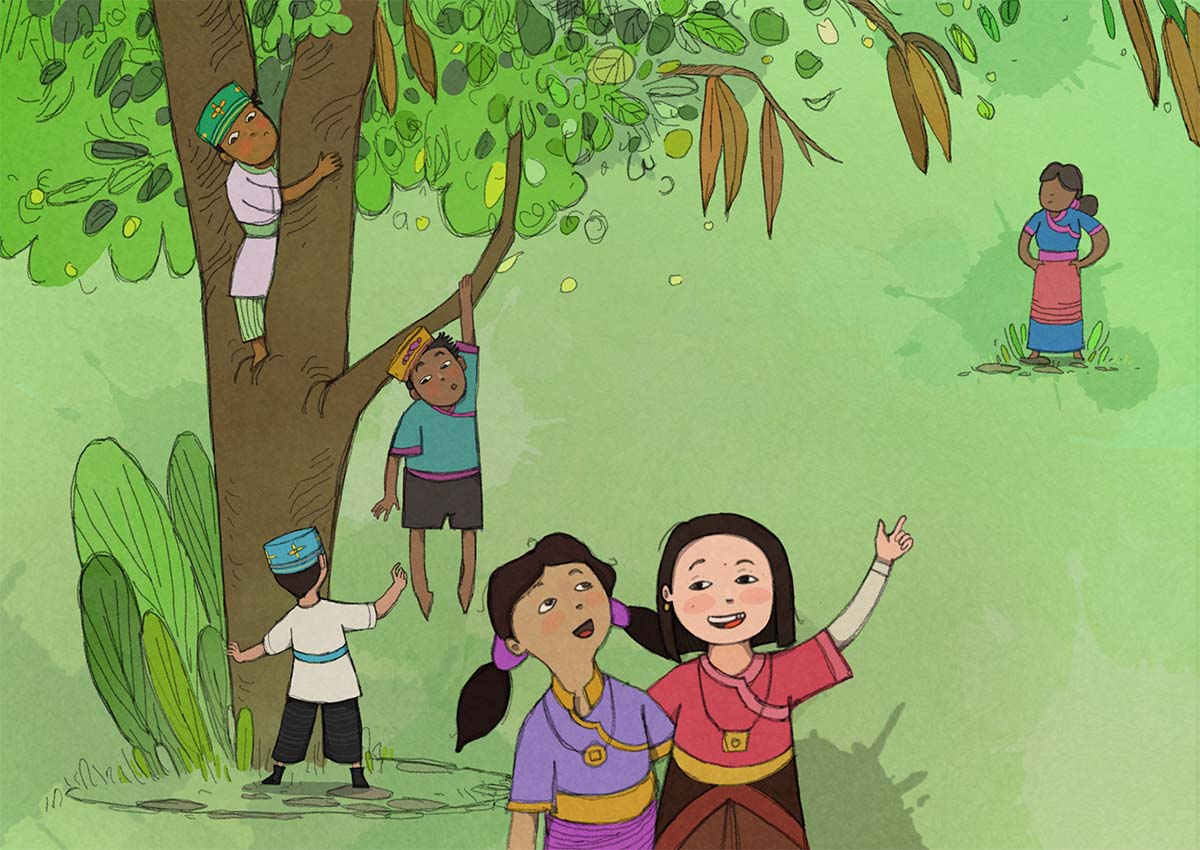
\includegraphics{images/p-3.jpg}

}

\end{figure}

\begin{longtable}[]{@{}l@{}}
\toprule\noalign{}
\endhead
\bottomrule\noalign{}
\endlastfoot
``लौ न बदमासहरूले सबै फूल नाश गर्नेभयो । सबै जना रुखबाट ओर्लि हाल त ।'' \\
\end{longtable}

\bookmarksetup{startatroot}

\hypertarget{section-2}{%
\chapter{}\label{section-2}}

\begin{figure}[H]

{\centering 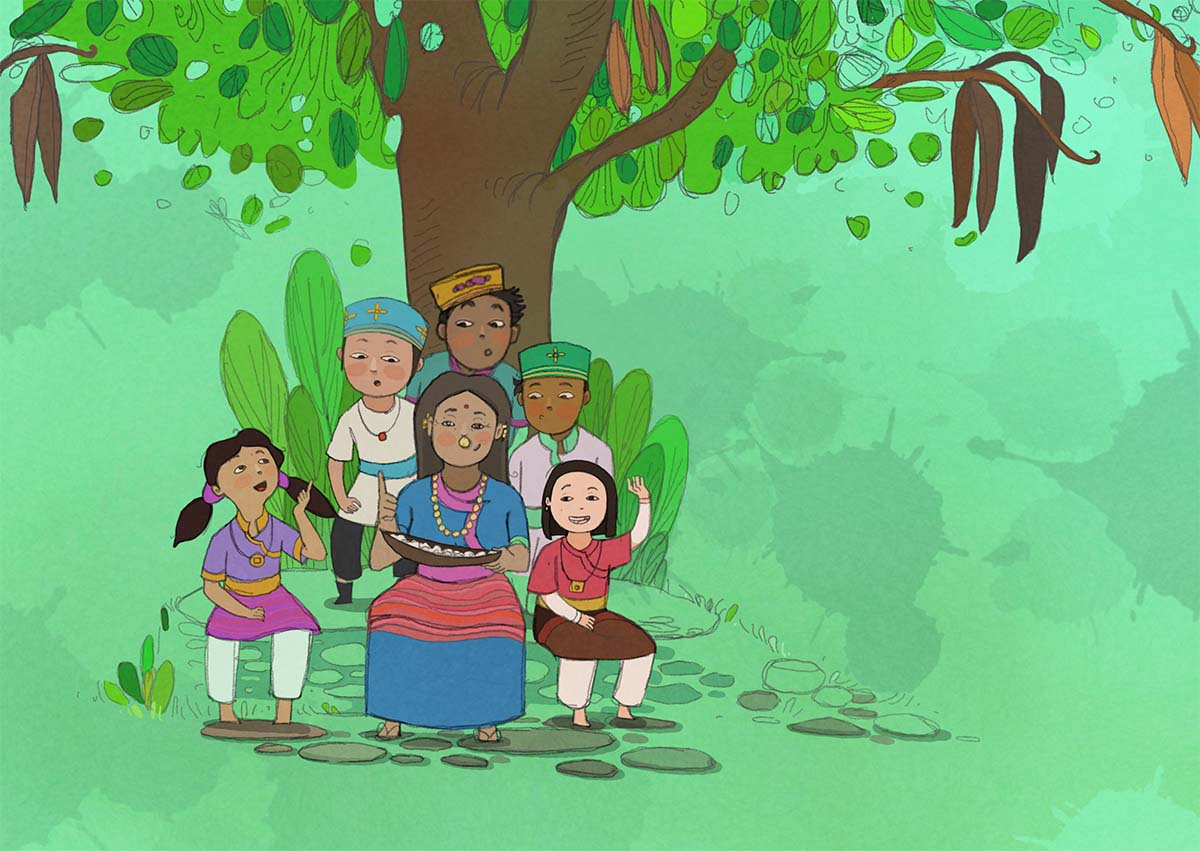
\includegraphics{images/p-4.jpg}

}

\end{figure}

\begin{longtable}[]{@{}l@{}}
\toprule\noalign{}
\endhead
\bottomrule\noalign{}
\endlastfoot
``हेर त ! यो टोटला चाेखाे फूल हो । यो खोलभित्र सपक्क मिलेको हुन्छ ।'' \\
\end{longtable}

\bookmarksetup{startatroot}

\hypertarget{section-3}{%
\chapter{}\label{section-3}}

\begin{figure}[H]

{\centering 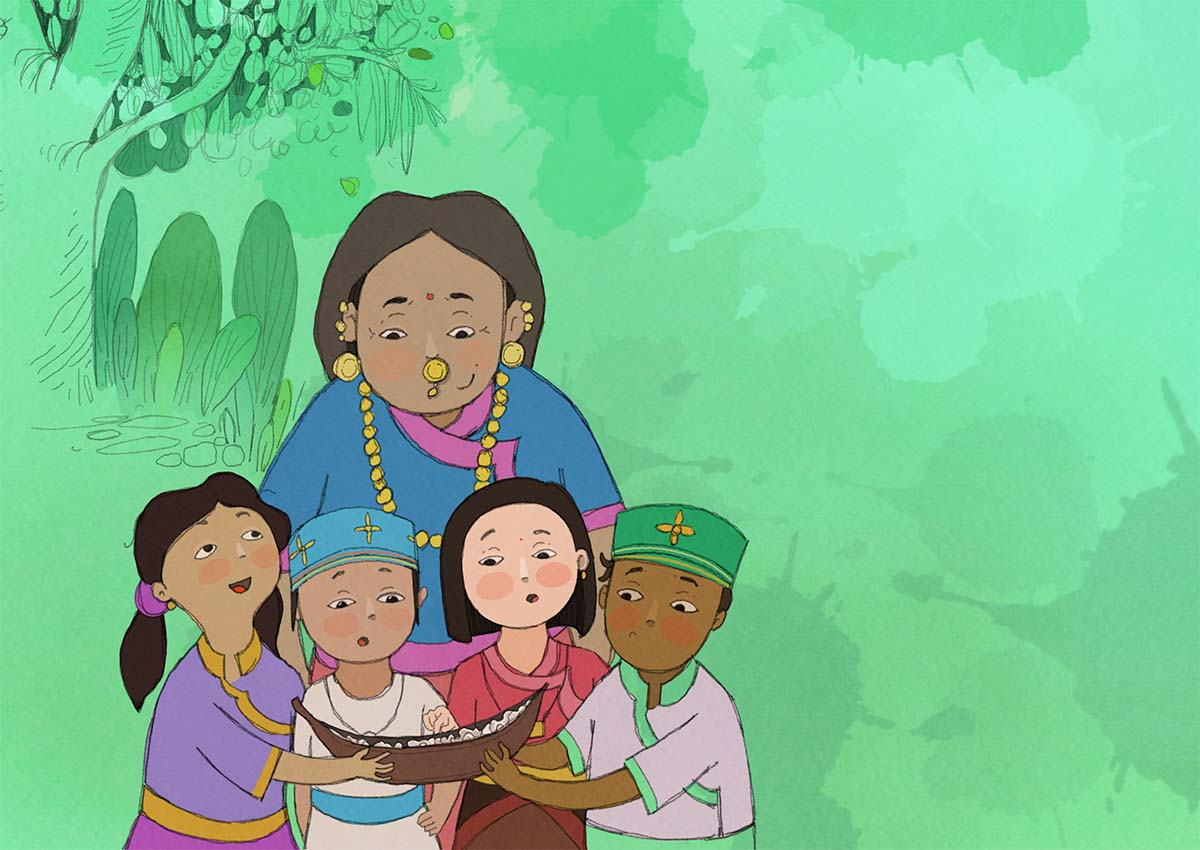
\includegraphics{images/p-5.jpg}

}

\end{figure}

\begin{longtable}[]{@{}
  >{\raggedright\arraybackslash}p{(\columnwidth - 0\tabcolsep) * \real{1.0000}}@{}}
\toprule\noalign{}
\endhead
\bottomrule\noalign{}
\endlastfoot
\begin{minipage}[t]{\linewidth}\raggedright
``आहा ! यसबाट माला पनि बन्छ ?''\\
``बन्छ ! बन्छ !''\strut
\end{minipage} \\
\end{longtable}

\bookmarksetup{startatroot}

\hypertarget{section-4}{%
\chapter{}\label{section-4}}

\begin{figure}[H]

{\centering 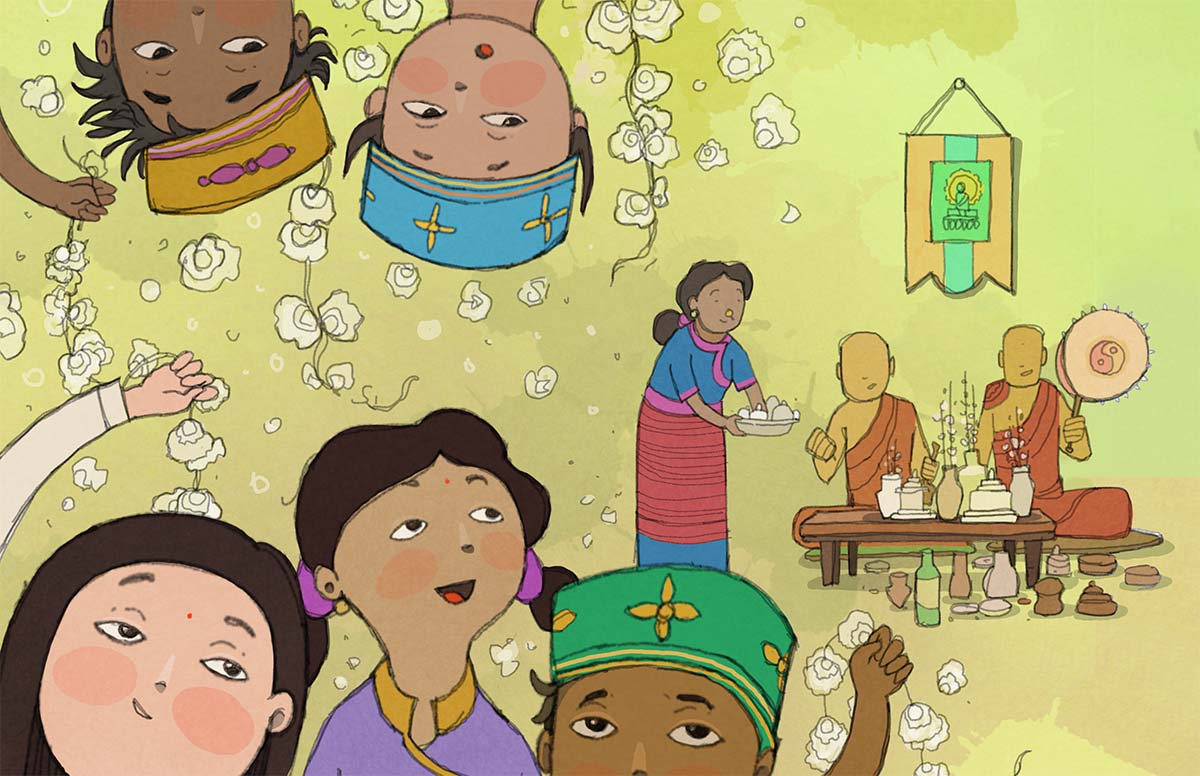
\includegraphics{images/p-6.jpg}

}

\end{figure}

\begin{longtable}[]{@{}l@{}}
\toprule\noalign{}
\endhead
\bottomrule\noalign{}
\endlastfoot
``हाम्रो पूजा, बिहे, छेवारमा नभई हुँदैन ।'' \\
\end{longtable}

\bookmarksetup{startatroot}

\hypertarget{section-5}{%
\chapter{}\label{section-5}}

\begin{figure}[H]

{\centering 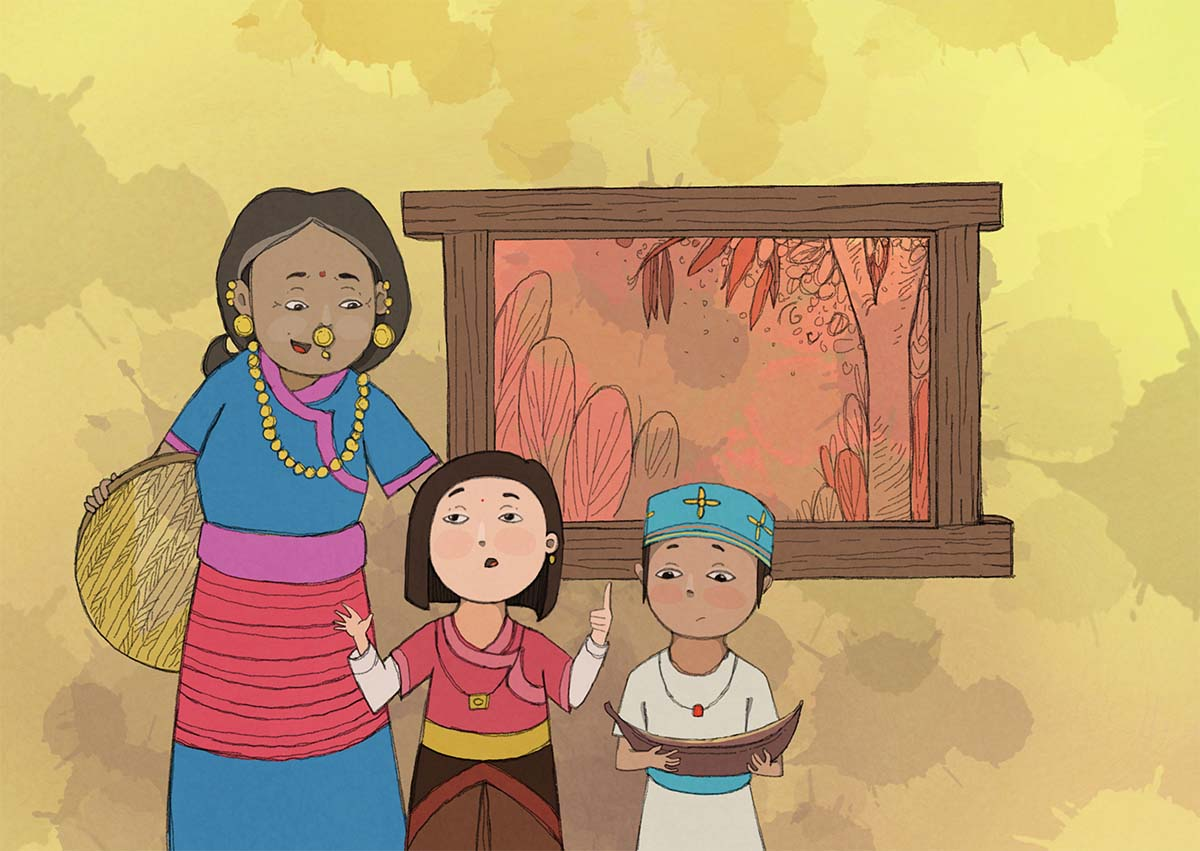
\includegraphics{images/p-7.jpg}

}

\end{figure}

\begin{longtable}[]{@{}l@{}}
\toprule\noalign{}
\endhead
\bottomrule\noalign{}
\endlastfoot
``हेर त, अब त टोटलाको फूल फुल्‍याजस्तो छ। जाऊ सबै जनालाई बोलाऊ'' \\
\end{longtable}

\bookmarksetup{startatroot}

\hypertarget{section-6}{%
\chapter{}\label{section-6}}

\begin{figure}[H]

{\centering 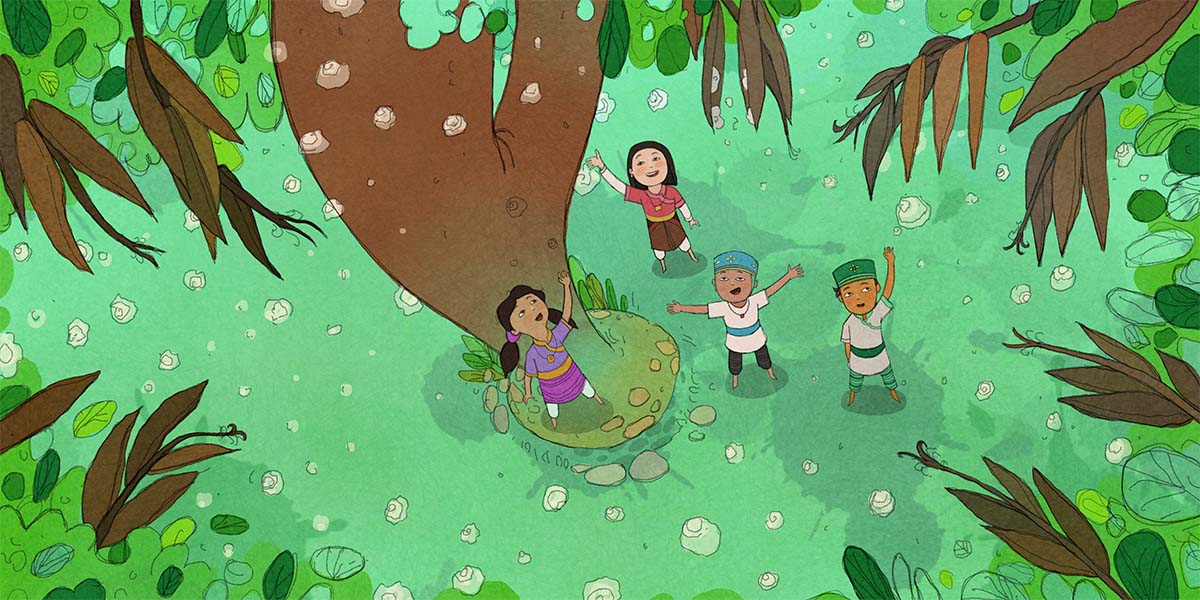
\includegraphics{images/p-8.jpg}

}

\end{figure}

\begin{longtable}[]{@{}
  >{\raggedright\arraybackslash}p{(\columnwidth - 0\tabcolsep) * \real{1.0000}}@{}}
\toprule\noalign{}
\endhead
\bottomrule\noalign{}
\endlastfoot
\begin{minipage}[t]{\linewidth}\raggedright
``ए उर्गेन ! साथीहरू खेल्न आइसके । म जाँदै गर्छु । तिमी छिट्टै आऊ ल !''\\
``ल नाना ल !''\strut
\end{minipage} \\
\end{longtable}

\bookmarksetup{startatroot}

\hypertarget{section-7}{%
\chapter{}\label{section-7}}

\begin{figure}[H]

{\centering 
\includegraphics{images/p-9.jpg}

}

\end{figure}

\begin{longtable}[]{@{}
  >{\raggedright\arraybackslash}p{(\columnwidth - 0\tabcolsep) * \real{1.0000}}@{}}
\toprule\noalign{}
\endhead
\bottomrule\noalign{}
\endlastfoot
यो पुस्तक All Children Reading: A Grand Challenge for Development (ACR
GCD) Founding Partners (the United States Agency for International
Development {[}USAID{]}, World Vision, र Australian Government) तथा
Global Book Alliance को संयुǣ सहयोगमा The Asia Foundation ले तयार गरेको
हो।यस पुस्तक मा सहयोगी संस्थाहरु ACR GCD Founding Partners वा Global Book
Alliance को ȱवचार प्रȱतȱबȸम्बत गदƺन। त्यसैले यस अनुकू लन अथवा अनुवाद कायर्लाई ACR
GCD Founding Partners र Global Book Alliance को कु नै पȱन हकमा आȲधकाȯरक
अनुकू लन वा अनुवाद माȱनने छैन साथै यस पुस्तकमा कु नै पȱन कथा वस्तु,सामग्री वा
त्रुȰटहरूको लाȱग उǶरदायी हुने छैन। \\
\end{longtable}

\bookmarksetup{startatroot}

\hypertarget{section-8}{%
\chapter{}\label{section-8}}

\begin{longtable}[]{@{}c@{}}
\toprule\noalign{}
\endhead
\bottomrule\noalign{}
\endlastfoot
\textbf{Brought to you by} \\
\end{longtable}

\begin{figure}[H]

{\centering 
\includegraphics{images/aflogo.png}

}

\end{figure}

\begin{longtable}[]{@{}
  >{\centering\arraybackslash}p{(\columnwidth - 0\tabcolsep) * \real{1.0077}}@{}}
\toprule\noalign{}
\endhead
\bottomrule\noalign{}
\endlastfoot
\begin{minipage}[t]{\linewidth}\centering
Let's Read is an initiative of The Asia Foundation's Books for Asia
program that fosters young readers in Asia and the Pacific.\\
\href{http://letsreadasia.org/}{booksforasia.org}\\
To read more books like this and get further information, visit\\
\href{http://letsreadasia.org/}{letsreadasia.org}.\strut
\end{minipage} \\
\end{longtable}

\begin{longtable}[]{@{}
  >{\raggedright\arraybackslash}p{(\columnwidth - 0\tabcolsep) * \real{1.0061}}@{}}
\toprule\noalign{}
\endhead
\bottomrule\noalign{}
\endlastfoot
\textbf{Original Story}

\emph{को म्हेन्दो,} Author: Shrijana Gole Tamang. Illustrator: Suman
Maharjan.

Published by The Asia Foundation - Let's
Read,~\href{https://letsreadasia.org/}{https://letsreadasia.org}~© The
Asia Foundation - Let's Read.~Released under CC-BY-4.0. \\
\end{longtable}

\begin{longtable}[]{@{}
  >{\raggedright\arraybackslash}p{(\columnwidth - 0\tabcolsep) * \real{1.0075}}@{}}
\toprule\noalign{}
\endhead
\bottomrule\noalign{}
\endlastfoot
This work is a modified version of the original story. © The Asia
Foundation, 2022. Some rights reserved. Released under CC-BY-4.0.


\includegraphics{images/ccby.jpg} For full terms of use and attribution,
\url{http://creativecommons.org/licenses/by/4.0/}

Contributing translators: Ritica Lacoul \\
\end{longtable}

\bookmarksetup{startatroot}

\hypertarget{references}{%
\chapter*{References}\label{references}}
\addcontentsline{toc}{chapter}{References}

\markboth{References}{References}

\hypertarget{refs}{}
\begin{CSLReferences}{0}{0}
\end{CSLReferences}



\end{document}
